\documentclass[12pt, aspectratio=169]{beamer}

\usepackage{minted}

\usetheme{metropolis}

\newcommand{\ferrisframe}[1]{%
  \begin{frame}[standout]
    
\includegraphics[height=0.8\textheight]{images/ferris.png}

    #1
  \end{frame}
}

\title{Introduction to Rust}
\date{December 12, 2017}
\author[@aqrln, @nechaido]{%
  \texorpdfstring{%
    \parbox{0.35\textwidth}{%
      Alexey Orlenko\\
      \href{https://twitter.com/aqrln}{@aqrln}
    }
    \parbox{0.35\textwidth}{%
      Dmytro Nechai\\
      \href{https://twitter.com/nechaido}{@nechaido}
    }
    \vspace{0.6cm}
  }
  {Alexey Orlenko, Dmytro Nechai}
}
\institute{HowProgrammingWorks}

\begin{document}

\maketitle

\ferrisframe{Lecture 1}

\begin{frame}{What is Rust}
  \begin{quote}
    ``Rust is a systems programming language that runs blazingly fast, prevents
    segfaults, and guarantees thread safety.''
  \end{quote}

  \rightline{\rm --- \url{https://www.rust-lang.org}}
\end{frame}

\begin{frame}{Rust's main strengths}
  \begin{itemize}
    \item safety
    \item speed
    \item concurrency
  \end{itemize}
\end{frame}

\begin{frame}{Rust's main features}
  \begin{itemize}
    \item Strong static typing with type inference
    \item Trait-based generics
    \onslide<2->{\item Functional programming features}
    \onslide<2->{\item Zero-cost abstractions}
    \onslide<3->{\item Guaranteed memory safety without GC}
    \onslide<3->{\item Threads without data races}
    \onslide<4->{\item Minimal runtime and C ABI}
  \end{itemize}
\end{frame}

\begin{frame}{Who is using Rust}
  \begin{columns}
    \column{0.25\textwidth}
    
\includegraphics[width=\textwidth]{images/mozilla.png}
    \column{0.25\textwidth}
    
\includegraphics[width=\textwidth]{images/dropbox.png}
    \column{0.25\textwidth}
    
\includegraphics[width=\textwidth]{images/atlassian.png}
  \end{columns}

  \begin{columns}
    \column{0.25\textwidth}
    
\includegraphics[width=\textwidth]{images/npm.png}
    \column{0.25\textwidth}
    
\includegraphics[width=\textwidth]{images/bitfury.png}
    \column{0.25\textwidth}
    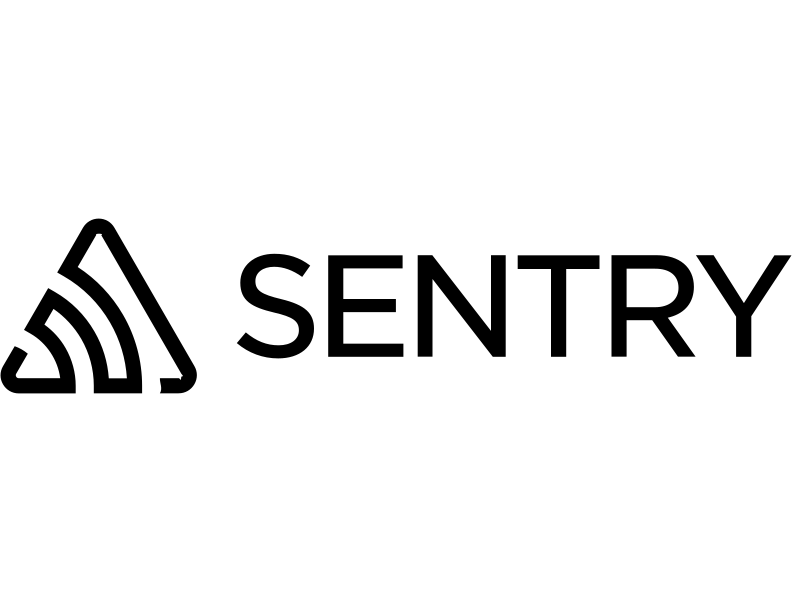
\includegraphics[width=\textwidth]{images/sentry.png}
  \end{columns}

  \begin{columns}
    \column{0.25\textwidth}
    
\includegraphics[width=\textwidth]{images/ovh.png}
    \column{0.25\textwidth}
    
\includegraphics[width=\textwidth]{images/coursera.png}
    \column{0.25\textwidth}
    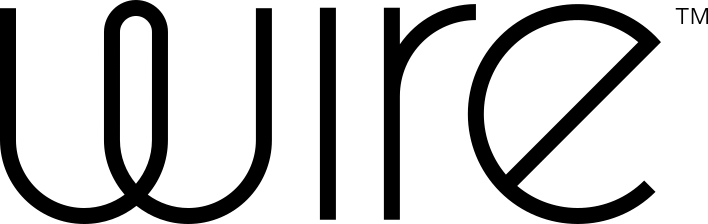
\includegraphics[width=\textwidth]{images/wire.png}
  \end{columns}
\end{frame}

\begin{frame}{Installing Rust}
  The official tool for managing Rust toolchains and their versions is
  \texttt{rustup}.

  \url{https://rustup.rs}
\end{frame}

\begin{frame}{Advantages for developers in languages like C or C++}
  \begin{itemize}
    \item Type and memory safety
    \item Zero-cost or low-cost high-level abstractions
    \item Standard tooling and package manager
  \end{itemize}
\end{frame}

\begin{frame}{Advantages for developers in languages like Python or JavaScript}
  \begin{itemize}
    \item Type and memory safety
    \item Performance
    \item Going lower-level without sacrificing expressiveness
  \end{itemize}
\end{frame}

\begin{frame}[fragile]{Hello World}
  \begin{minted}{rust}
  fn main() {
    println!("Hello!");
  }
  \end{minted}
\end{frame}

\begin{frame}{Resources for learning Rust}
  \begin{itemize}
    \item ``The Rust Programming Language'' Book \only<2>{---\\
      \url{https://doc.rust-lang.org/book/}}
    \item Rustonomicon \only<3>{---\\ \url{https://doc.rust-lang.org/nomicon/}}
    \item Unstable Book \only<4>{---\\
      \url{https://doc.rust-lang.org/beta/unstable-book/}}
    \item Reference \only<5>{---\\ \url{https://doc.rust-lang.org/reference/}}
  \end{itemize}
\end{frame}

\ferrisframe{Thanks for coming and see you next time!}

\end{document}
